\chapter{Week 1: Webserver}

\section{Ethernet Shield}\index{Ethernet Shield}

We beginnen dit hoofdstuk met de laatste opdracht van \textit{Programmeren 1}, de “uitsmijter” van de introductie in embedded systems en embedded programming: de Arduino met IO-webserver.

\subsection*{inleiding}
Als onderdeel van de Arduino software worden diverse software-componenten meegeleverd in de vorm van software-bibliotheken ($libraries$) (Je kunt ze onder Windows vinden onder: $Mijn Documenten$ -> $Arduino$ -> $libraries$). Controleer dat. Standaard wordt er, bijvoorbeeld, een servo-library meegeleverd waarmee het werken met servo’s sterk wordt vereenvoudigd. Deze libraries kun je in je code gebruiken door ze zogeheten te $includen$, dit doe je door bovenaan in je code de volgende regel toe te voegen:

\begin{lstlisting}[language=Arduino]
#include <NaamVanLibrary.h>
\end{lstlisting}

Daarna kun je alle handige functies die in de library zitten gebruiken in je eigen code. Op de volgende manier kun je bijv. voor de ethernet-shield een webserver worden geconfigureerd, door gebruik te maken van de $Ethernet$-library: \newline

\lstinputlisting[language=Arduino]{code/chapter01/webserver.ino}

Om daadwerkelijk met de ethernet-shield een connectie te krijgen, is de library wat informatie van je nodig. Op regel $6$, wordt een $EthernetServer$ 'object' aangemaakt met de naam $server$ en deze krijgt ook het getal $80$ mee. Dit is het poort-nummer waarmee je gaat werken, gezien dat we iets met $http$ ('het internet') gaan doen, is dit $80$ (deze poort is daarvoor gereserveerd). Voor meer informatie over dit $http$ protocol\: \url{http://betterexplained.com/articles/a-simple-introduction-to-computer-networking/}. \newline

Je router (die alle verkeer in je netwerk beheert) heeft daarnaast informatie nodig van het apparaat zodat deze data daar naartoe kan sturen. Vergelijkbaar met je woonaddress, heeft zo'n apparaat ook een addres, twee zelfs! Een MAC-address (die vaak bestaat uit 6 hexadecimale getallen), die uniek moet zijn voor elk apparaat in het netwerk. Vaak worden de ethernetshields geleverd met een sticker waar een uniek (gereserveerd) MAC-address opstaat, mocht dit voor jou nu niet het geval zijn, vul dan iets willekeurigs in (we sluiten de Arduino enkel aan op het lokale netwerk, dus de kans dat er in dat kleine netwerk een dubbele voorkomt is nagenoeg nihil). \newline 
Het IP-adres bestaat uit 4 getallen, vaak in de trant van $192.168.1.X$ (of bijv. $10.0.0.X$), waarbij $X$ het computernummr is, wat een uniek getal moet zijn in je lokale netwerk. Deze addressen worden gebruikt om een connectie te maken tussen apparaten in het lokale netwerk. Beide worden dan ook 'meegegeven' bij het aanroepen van de $begin()$ functie van de $Ethernet$-library, deze zorgt dat alle nodige configuratie verder wordt uitgevoerd om met het ethernetshield aan de slag te gaan. \newline

\subsection{Opdrachten}
\begin{exercise}
$\\$ Plaats de Arduino ethernetshield op de Arduino UNO en download het bijbehorende programma (Arduino script, iowebserver.ino) via blackboard en laadt het in je Arduino.
\end{exercise}

\begin{remark}
Let op: als je het ethernetshield op je Arduino aansluit, zijn de pins 10 - 13 niet meer te gebruiken voor andere doeleinden.
\end{remark}

\begin{exercise}
$\\$ Sluit je ethernetshield aan op je laptop of (beter nog) op een router, waar uiteraard ook je laptop aan hangt (bedraad of draadloos). \newline
Onderzoek wat het IP-adres van je laptop is en noteer dit. \newline 
(Merk op dat je laptop naast de bedrade aansluiting ook nog verbonden kan zijn met het internet via de draadloze verbinding. Dat is handig, want dan kun je ondertussen stackoverflow raadplegen.) \newline \newline 
Een directe verbinding tussen twee systemen noemt men een ad hoc-netwerk. In beide gevallen, ad hoc of via een router, is het verstandig de netwerkadressen te kiezen in het segment $192.168.1.x$, waarbij $x$ het computernummer is. Het voordeel van dit segment is dat het strikt lokaal is. De informatie van computers in dit segment worden niet doorgegeven over het internet. 
\end{exercise}

\newpage
\begin{exercise}
$\\$ Bestudeer het webserver-programma en onderzoek of je webserver een IP-adres krijgt en zo ja, welke? \newline
Gebruik de Serial Monitor. Noteer dit adres ook en vergelijk het met dat van je laptop. \newline 
Zitten beide systemen in hetzelfde netwerk(segment)? \newline \newline

De toekenning in de Arduino kan statisch of dynamisch, via DHCP. Welke gebruik je? \newline 
Zorg er hierbij voor dat je in een gecontroleerde netwerkomgeving werkt, met bijvoorbeeld een eigen router waarvan je de instelling kunt aanpassen. \newline
Op het NHL-netwerk hebt je weinig vat, wat aanleiding kan vormen tot problemen (met firewalls etc.). Bij de statische configuratie bepaal je zelf wat het IP-adres is. Je kunt het (in Windows) aanpassen via het configuratiescherm. \newline
Een nadeel van een statisch IP is dat je, in een netwerk met meerdere computers, conflicten kunt krijgen. Beter is het dan ook je Arduino via DHCP een IP-adres te laten toekennen. Dit wordt ondersteund door de serversoftware.
\end{exercise}

\begin{remark}
Voor de rest van deze opgave gaan we uit van de volgende configuratie: de laptop krijgt adres $192.168.1.2$ en de Arduino(server) $192.168.1.3$. Dat kan bij jou dus, zeker als je DHCP gebruikt, anders zijn. \newline
\end{remark}

Probeer, nu je begrijpt hoe eenvoudige netwerkcommunicatie werkt, de Arduino file $webserver.ino$ te downloaden van BlackBoard en in de Arduino te ladan. Als dit is gelukt, is de webpagina, via je browser zichtbaar te maken door de volgende URL in de voeren:\newline
\url{http://192.168.1.3} \newline
Zie figuur \ref{fig:webserver} voor hoe de site eruit hoort te zien. Mocht dit niet gebeuren en je weet zeker dat alle IP-adressen kloppen, lees dan verder bij de opmerking onderaan deze opdracht.

\begin{figure}[h!]
\centering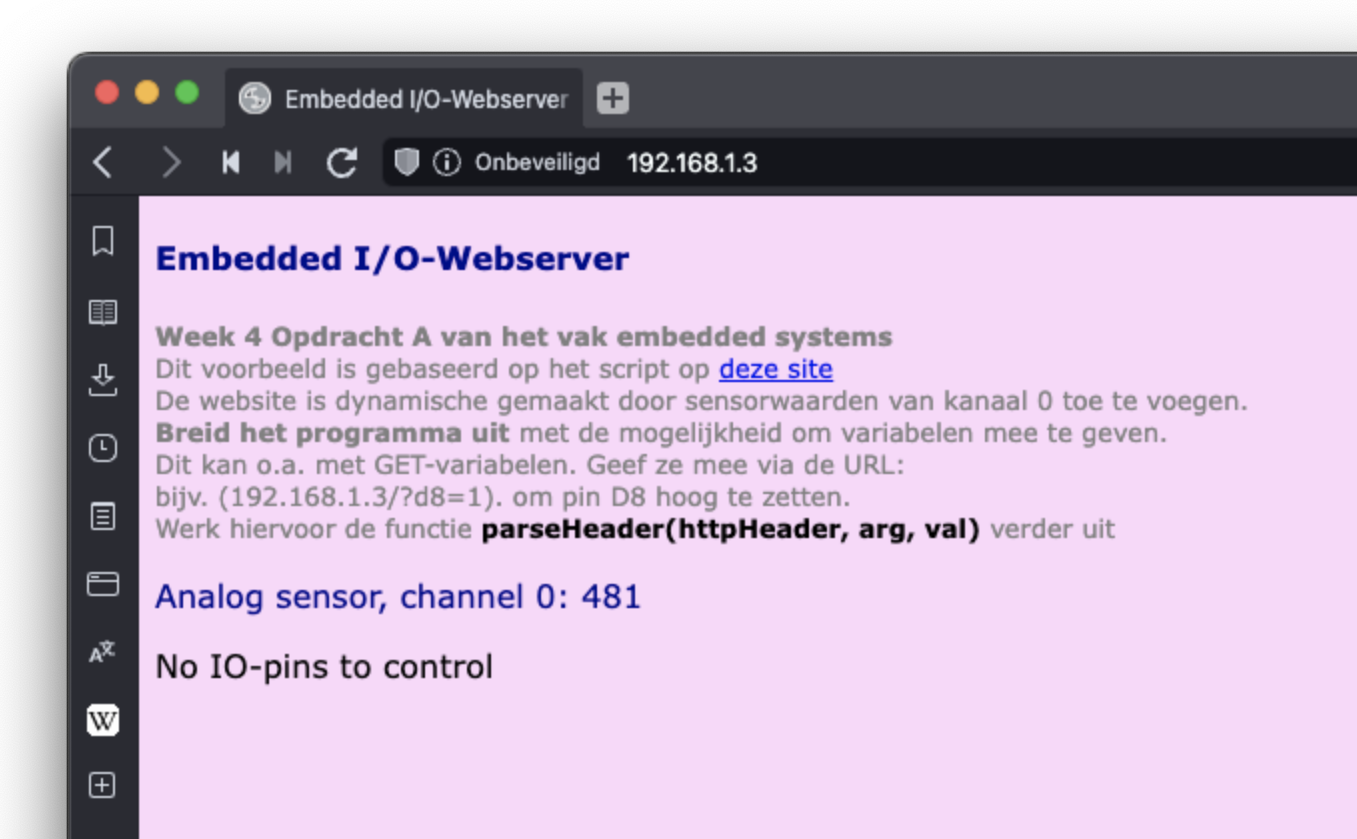
\includegraphics[scale=0.25]{Pictures/chapter01/webserver.png}
\caption{Webserver}
\label{fig:webserver} % Unique label used for referencing the figure in-text
%\addcontentsline{toc}{figure}{Figure \ref{fig:webserver}} % Uncomment to add the figure to the table of contents
\end{figure}

\begin{exercise}
Sluit een sensor aan op je Arduino (bijvoorbeeld een lichtsensor of een potmeter op kanaal $A0$) en modificeer je programma zodanig dat je uitsluitend de sensorwaarde, en niet de hele string “Analog sensor (channel 0): ”, bold (vetgedrukt) afdrukt en kleur deze daarnaast rood indien deze boven de $600$ komt. Onderzoek de mogelijkheid om dit automatisch te herhalen elke 3 seconden. \textit{Hint:} Meta Tag.\newline
Gebruik zo nodig: \newline
\url{http://www.w3schools.com/html http://www.w3schools.com/cssref/css_colornames.asp}
\end{exercise}

\section{Hoofdopdracht: Webserver}

\begin{exercise}
Pas je programma zodanig aan dat je via een zogeheten 'GET-variabele' (als onderdeel van je URL) de server opdracht kunt geven de afzonderlijke LED’s aan de pinnen $p8$ en $p9$ aan en uit kunt zetten. \newline \newline Daarmee bedoelen we dat het aanpassen je je gebruikte url (het IP-adres van de Arduino): \newline
\url{http://192.168.1.3/} \newline
naar bijv: \newline
\url{http://192.168.1.3/?p8=1} \newline
Waarmee de LED aan pin 8 aan wordt aangezet. Overeenkomstig kan met \newline
\url{http://192.168.1.3/?p9=0} \newline
de LED aan pin 9 worden uitgezet (terwijl die aan pin 8 natuurlijk aan blijft). \newline \par
Zoek onderin je code naar de functie $parseHeader()$, hier moet de URL van hierboven worden verwerkt ($geparsed$). 

\begin{lstlisting}[language=Arduino, numbers=none]
bool parseHeader(String header, int &a, int &v)
{
   // your code goed here 
}
\end{lstlisting}
Vul deze functie in zodat deze de url (na het vraagteken) splits in een argument (in ons geval: $p8$ of $p9$) en een waarde ($0$ of $1$). Sla het argument op in $a$ en de waarde in $v$. 

\begin{remark}
De parameters $a$ en $v$ zijn uitvoer-parameters (of reference parameters). Een toekenning, binnen de functie, van een waarde aan één van de beide parameters leidt tot een aanpassing van de argumenten (variabelen) bij aanroep. Kortom: verander je $a$, dan verandert $arg$ dus mee. Dat is de essentie van \textit{call by reference}. 
\end{remark}

Meld de gebruiker (via de website) de veranderingen in de status van de beide pinnen, ook als er zich fouten voordoen.
\end{exercise}

\subsection{Verdieping (optioneel)}
\begin{exercise}
Plaats een SD-card in je ethernetshield en laadt de webpagina van SD-card.
\end{exercise}

\begin{exercise}
Breng de Arduino ter sprake als de gesprekken, thuis aan tafel of in de kroeg stilvallen. Doe dit met dermate veel enthousiasme dat vriendinnen, jongere broertjes en neefjes ook informatica willen gaan studeren ;)
\end{exercise}

\newpage

\section{Optionele opdracht: Webclient}
In de vorige opdracht hebben we gezien hoe de Arduino tijdelijk is omgetoverd tot een eenvoudige webserver waarmee, via het http-protocol, sensoren uitgelezen kunnen worden en hardware bestuurd kan worden. In deze opdracht gaan we de rollen omdraaien. We gaan met de Arduino, wederom via http, gegevens van een (externe) website of webserver opvragen. Dit gaat via een http request waarbij de Arduino nu in de rol van client optreedt (vergelijkbaar met wat een browser doet). \par 
We gaan ook onderzoeken hoe snel die gegevensoverdracht eigenlijk is (in termen van Bytes/s). \newline \newline

De basis voor deze opdracht komt van de Arduino-site: \newline
\url{https://www.arduino.cc/en/Tutorial/WebClient} \newline
Dit voorbeeld maakt duidelijk hoe je een http request uitvoert met gebruik van een ethernet shield en daarbij gegevens opvraagt van een google server. \newline \newline

\begin{exercise}
Download de code van deze website en sla deze op onder de naam $WebClient.ino$. Bestudeer de code. Enkele opmerkingen daarover:
\begin{lstlisting}[language=Arduino, numbers=none]
// Set the static IP address to use if the DHCP fails to assign
IPAddress ip(192, 168, 0, 177);
IPAddress myDns(192, 168, 0, 1);
\end{lstlisting}

Pas deze gegevens aan aan je eigen (thuis)situatie.
\end{exercise}

\begin{remark}\textit{Let op}: in de code wordt in eerste instantie geprobeerd een IP-adres te verkrijgen via DHCP. Lukt dat niet dan wordt teruggevallen op een statisch IP-adres. Dat geldt ook voor de optie om met DNS te werken zodat je niet via het IP-adres een google-site benadert, maar via de URL. Je kunt de DNS van je router gebruiken, dat is (doorgaans) de gateway naar je provider. Bij het verkrijgen van een IP-adres kan het programma nog onderscheid maken tussen diverse foutsituaties, zoals die waarbij er geen shield of geen ethernet kabel is aangesloten. Handig! Helaas wordt dat niet door elke ethernet-chip ondersteunt, wat bij correcte aansluiting verder geen problemen oplevert.
\end{remark}

\begin{lstlisting}[language=Arduino, numbers=none]
EthernetClient client;
\end{lstlisting}

De variabele $client$, via welke het verdere interface verloopt is van het type $EthernetClient$. Deze is bekend, en daardoor oranje in de code, via het include statement, bovenin het programma.

\begin{lstlisting}[language=Arduino, numbers=none]
Ethernet.begin(mac, ip, myDns);
\end{lstlisting}

\begin{remark}
\textit{Let op}: $Ethernet$ is feitelijk de abstractie van de shield. Via dit object hebben we toegang tot de shield. Uiteraard heeft dit object methoden, zoals $begin()$, waarmee de shield wordt geïnitialiseerd. $begin()$ heeft meerdere verschijningsvormen of interfaces. Eén met alleen een mac-adres of één met een mac-adres en een IP-adres. De hier gekozen variant gaat uit van een DNS-adres zodat de server via een URL kan worden benaderd. Voor meer informatie, zie bij: \newline
\url{https://www.arduino.cc/en/Reference/EthernetBegin}
\end{remark}

Eenmaal (goed) geïnitialiseerd kan het lokale IP-adres worden afgedrukt met:

\begin{lstlisting}[language=Arduino, numbers=none]
Serial.println(Ethernet.localIP());
\end{lstlisting}

Daarna wordt er gepoogd een verbinding met een externe server te maken, met:
\begin{lstlisting}[language=Arduino, numbers=none]
if (client.connect(server, 80))
\end{lstlisting}
Merk op dat connect een methode is van het client object, dat server een argument is dat hieraan meegegeven wordt en dat server , i.v.m. de DNS-optie, hier een URL is. Dat is hier een (statische) string. Zie bovenin het programma. Je kunt, via out-commenting, ook kiezen voor een ‘hard’ IP-adres, als de DNS-optie niet werkt. \par
Eenmaal verbonden met de server, kun je het IP-adres, nu van de server, opvragen en printen met 
\begin{lstlisting}[language=Arduino, numbers=none]
Serial.println(client.remoteIP());
\end{lstlisting}

Daarna voert het programma zijn taak uit. Dat begint met:
\begin{lstlisting}[language=Arduino, numbers=none]
client.println("GET /search?q=arduino HTTP/1.1");
\end{lstlisting}

waarin, vanuit de setup code, de feitelijke http request wordt gedaan, waarna de bijbehorende http response, in de loop code, wordt verwerkt. In dit geval betekent dat, dat zolang de $client.available()$ is, het lezen van de reactie van de server, met een mogelijkheid tot printen en het tellen van het aantal gelezen bytes, zodat, op grond daarvan en van een tijdcriterium, kan worden vastgesteld wat de overdrachtssnelheid is. Merk op dat voor het meten van de leestijd de functie $micros()$ wordt gebruikt. Deze snelheid wordt doorgaans uitgedrukt in MB/s, maar vanwege de relatieve traagheid van de Arduino hier in kB/s. Let op (alweer), dat het printen van de response een grote invloed heeft op deze snelheid. Beredeneer waarom dat zo is? Voor een betrouwbaarder meting is het dan ook raadzaam het printen uit te zetten.
Oh ja, misschien is dit een goed moment om de baudrate van de Arduino ($Serial.begin$) aan te passen van 9600 bps (bits/s) naar 115200 bps, zowel in de code als in het serial monitor. 115200 bps komt neer op ongeveer 11000 tekens per seconde. Dat kan de Arduino wel aan, maar jij, wat betreft leessnelheid, waarschijnlijk niet ;)
Voer de code uit en stelt vast wat de google-server terugstuurt (bij zoeken op de term “Arduino”) en wat de overdrachtsnelheid hierbij is. \newline \newline

Het programma is in deze vorm slechts geschikt voor één taak. Vaak is het realistisch dat er meerdere requests gedaan moeten worden, bij meerdere servers. Daarover straks meer. Om dat voor te bereiden is het nodig om het request en de response in één functie uit te voeren.

\begin{exercise}
Modificeer het programma zodanig dat deze functionaliteit wordt uitgevoerd door de functie $speedTest$, waarvan deze functie-header wordt gebruikt:

\begin{lstlisting}[language=Arduino, numbers=none]
void speedTest(bool doPrint = false);
\end{lstlisting}
Een mogelijke aanroep van deze functie is speedTest()waarbij het printen standaard uitstaat. Hier wordt gebruik gemaakt van de mogelijkheid een parameter in de heading een initiële waarde te geven. De koppeling van de waarde aan de variabele vindt plaats tijdens de aanrop. Een andere mogelijkheid is deze:
\begin{lstlisting}[language=Arduino, numbers=none]
#define PRINT true // let op de conventie van hoofdletters 
speedTest(PRINT);
\end{lstlisting}
waarmee bij aanroep bepaald kan worden of de speedtest-functie wel of niet de response laat zien. Defines worden meestal helemaal boven in het programma opgenomen, in hoofdletters.\newline 

Wat moet de functie precies doen? Vier deelfuncties: 
\begin{enumerate}
  \item[1] verbinding met de server maken
  \item[2] uitvoeren van de http request (GET)
  \item[3] het verwerken van de respeonse van de server
  \item[4] het afhandelen van de timing en de speed-berekeningen
\end{enumerate}
\end{exercise}

Opmerkingen:
\begin{enumerate}
  \item[-] De eenmalige handelingen voor het initialiseren van het ethernet shield blijven,logischerwijs, in de setup code.
  \item[-] Alle variabelen gerelateerd aan deze functies worden uiteraard lokaal gehouden, dus binnen de functie gedefinieerd. Dat geldt voor: $beginMicros$, $endMicros$, $byteCount$ en ook de $buffer$ en $len$.
  \item[-] Dit klinkt als een eenvoudige opdracht (en dat klopt, het is ook niet zo moeilijk), maar goed programmeren begint met een strikte scheiding in functies, het parameteriseren daarvan (zodat bij de aanroep het gedrag van de functie beïnvloed kan worden) en met met het vermijden van globale variabelen. Er zijn nog wel meer criteria te geven, maar voor nu is dit wel even voldoende.
  \item[-] Nog een belangrijk punt van aandacht: het bestaande programma maakt gebruik van het herhalende karakter van de functie loop. Dat raken we (bewust) kwijt door deze aanpassing. Loop blijft hier voorlopig leeg. Dat betekent dat je zelf een oplossing moet bedenken de noodzakelijke herhaling bij het lezen van de response. Dat gaat namelijk in regel (van max. 80 tekens). \newline
Een ander punt daarbij is: wanneer is het lezen klaar? Wanneer is de gehele response van de server verwerkt? Daarbij doemen ook de vragen op, als: wanneer wordt de verbinding verbroken en wie is daarvoor verantwoordelijk? Hint:
  \begin{enumerate}
    \item[-] kijk naar $client.connected()$
    \item[-] overweeg dit te gebruiken: $while (buflen = client.available() > 0)$ Dat mag in C: het toekennen van het functieresultaat aan een lokale variabelen en het (bijna) tegelijkertijd testen van deze variabelen, in dit geval op groter dan 0, waarmee wordt aangegeven dat er nog steeds iets te lezen valt.
    \item[-] zet om de read-actie even een digitalWrite, zodat je een visuele feedback krijgt in de vorm van een knipperend ledje.
  \end{enumerate}
\end{enumerate}
\begin{exercise}
Test je programma op juiste werking. Welke speed haal je?
\end{exercise}

\subsection{Verdieping (optioneel)}
\begin{exercise}
parameterisering, zeker bij klassiek, gestructureerd programmeren in een functionele taal, een sterk middel om je programma overzichtelijk en flexibel te houden. Ook het streven naar zo generiek mogelijke functies en oplossingen hoort daarbij. Ontwerp en functie, bijvoorbeeld httpRequest, die generieker is en waarbij je niet alleen print-criterium meegeeft, maar ook de url en de server en het antwoord, bijvoorbeeld als JSON-string, laat opleveren als functieresultaat.
\end{exercise}

\begin{exercise}
  http request zijn erg handig om data of informatie van verschillende servers te halen en te verwerken in je programma. Onderzoek de mogelijkheid om dat te doen voor bijvoorbeeld weer-informatie (bij \url{openweathermap.org}) of nieuws (bij \url{newsapi.org}). Je kunt deze gegevens, in een embedded systeem, tonen op bijvoorbeeld een displaytje.
\end{exercise}

